\subsection{RAT-SQL}

\begin{figure}[htb]
    \centering
    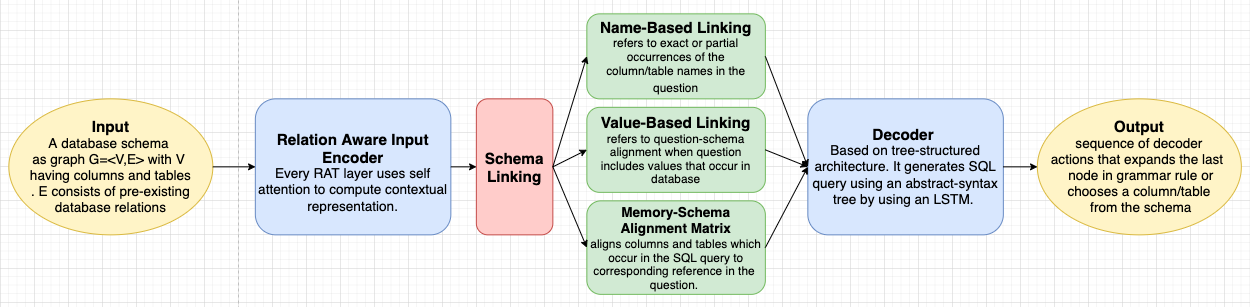
\includegraphics[width=0.8\textwidth]{pics/RAT-SQL/flow.png}
    \caption{A flow chart of RAT-SQL model}
    \label{fig:RAT-SQL-flow}
\end{figure}

\begin{itemize}
    \item A major challenge in translating natural language queries into SQL queries is generalizing them to unknown database schemas.
    \item As part of the generalisation, it is necessary to encode database relations in an accessible way and model alignment between relevant database columns in the query.
    \item Within a text2SQL encoder, the proposed framework leverages the relation-aware self-attention mechanism to encode address schemas, represent features, and link schemas.
    \item Check out the flow chart below for an overview of RAT-SQL's encoder-decoder structure.
\end{itemize}

\begin{figure}[htb]
    \centering
    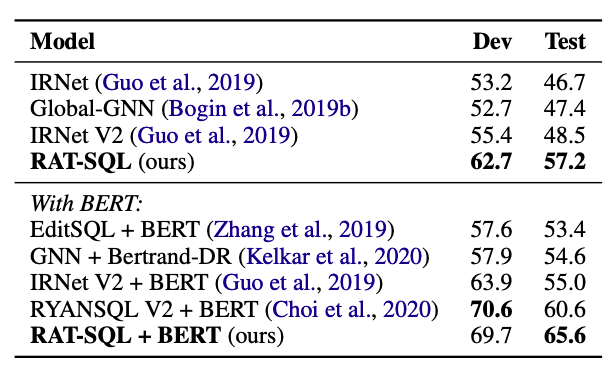
\includegraphics[width=0.4\textwidth]{pics/RAT-SQL/Accuracy.png}
    \caption{Accuracy on the Spider development and test sets, compared to the other approaches at the top of the dataset leaderboard as of May 1st, 2020 from \cite{wang_rat-sql_2021}}
    \label{fig:RAT-SQL-Accuracy}
\end{figure}

On the SPIDER dataset, RAT-SQL achieves 57.2\% accuracy, an improvement of 8.7\% over previous benchmark models.

\begin{figure}[htb]
    \centering
    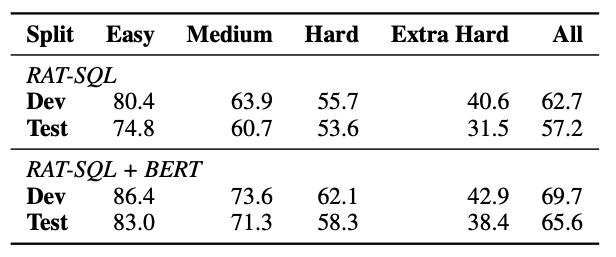
\includegraphics[width=0.4\textwidth]{pics/RAT-SQL/Accuracy2.png}
    \caption{Accuracy on the Spider development and test sets, by difficulty from \cite{wang_rat-sql_2021}}
    \label{fig:RAT-SQL-Accuracy2}
\end{figure}

With RAT-SQL, 65.6\% accuracy can be achieved by combining BERT with RAT-SQL.
